\documentclass{article}

\usepackage{graphicx} % Required for inserting images
\usepackage{mathtools}
\usepackage[hidelinks]{hyperref}
%\usepackage{bbm}  % for \mathbb and \mathbbm symbols
\usepackage{amsmath,amsfonts,amssymb, amsthm}
\usepackage{cleveref} % this needs to go after hyperref and amsmath

%\usepackage[chapter]{algorithm}  % for algorithm environment, option: use chapters for numering
\usepackage{tikz}
\usetikzlibrary{positioning}

\usepackage{tikz-cd}  % commuting diagrams based on tikz
\usetikzlibrary{calc}
\usepackage{booktabs}  % for clean tables (tabular environment) 
\usepackage{caption}  % for setting caption width
\captionsetup{width=\linewidth}

\definecolor{Green}{rgb}{0, 0.5, 0.2}
\usepackage[dvipsnames]{xcolor}
\usetikzlibrary{decorations.markings}

\usepackage{titlesec}
\titleformat{\chapter}[display]
  {\normalfont\huge\scshape}
  {\thechapter}
  {0.5em}
  {}
  [\vspace{0.5ex}\titlerule]

% Section
\titleformat{\section}
  {\normalfont\Large\scshape}
  {\thesection}
  {0.5em}
  {}

% Subsection
\titleformat{\subsection}
  {\normalfont\large}
  {\thesubsection}
  {0.5em}
  {}

\captionsetup{width=\textwidth, labelfont=bf, font=small}

\definecolor{greenii}{RGB}{20,140,10}
\definecolor{darkgreen}{rgb}{0.00,0.85,0.1}

\newcommand{\red}[1]{{\color{red} {#1}}}
\newcommand{\orange}[1]{{\color{orange} {#1}}}
\newcommand{\blue}[1]{{\color{blue} {#1}}}
\newcommand{\green}[1]{{\color{OliveGreen} {#1}}}

\usepackage[backend=biber, maxbibnames=3,style=alphabetic, backref,backrefstyle=none]{biblatex}
\addbibresource{bachelors.bib}

\AtEveryBibitem{
  \clearfield{issn}
  \clearfield{language}
  \clearfield{note}
  \clearfield{urldate}
}

\AtEveryBibitem{%
  \ifboolexpr{
    ( test {\ifentrytype{article}} or test {\ifentrytype{online}})
    and
    ( not test {\iffieldundef{doi}} or not test {\iffieldundef{eprint}} )
  }
  {\clearfield{url}}
  {}
}

\AtEveryBibitem{%
  \ifboolexpr{
    not test {\iffieldundef{doi}}
    or not test {\iffieldundef{eprint}}
  }
  {\clearfield{url}}
  {}
}

\newcommand{\ket}[1]{\ensuremath{\left| #1 \right\rangle}}
\newcommand{\bra}[1]{\ensuremath{\left\langle #1 \right|}}
\newcommand{\braket}[2]{\ensuremath{\left\langle #1 \middle| #2 \right\rangle}}
\newcommand{\ketbra}[2]{\ensuremath{\left| #1 \right\rangle \left\langle #2 \right|}}
\newcommand{\braopket}[3]{\ensuremath{\left\langle #1 \middle| #2 \middle| #3 \right\rangle}}

\newcommand{\SU}[1]{\mathrm{SU}(#1)}
\newcommand{\SO}[1]{\mathrm{SO}(#1)}
\newcommand{\U}[1]{\mathrm{U}(#1)}
\newcommand{\Sp}[1]{\mathrm{Sp}(#1)}
\newcommand{\GL}[1]{\mathrm{GL}(#1)} % e.g., GL(n, R)
\newcommand{\SL}[2]{\mathrm{SL}(#1, #2)}

\newcommand{\liesl}[1]{\mathfrak{sl}_{#1}} % sl_2 lie algebra.

%\theoremstyle{italics}
\newtheorem{theorem}{Theorem}[section]
\newtheorem{lemma}[theorem]{Lemma}
\newtheorem{fact}[theorem]{Fact}
\newtheorem{conjecture}[theorem]{Conjecture}
\newtheorem{proposition}[theorem]{Proposition}
\newtheorem{corollary}[theorem]{Corollary}
\theoremstyle{definition}
\newtheorem{definition}[theorem]{Definition}
\newtheorem{notation}[theorem]{Notation}
\newtheorem{literature}[theorem]{Literature}
\newtheorem{example}[theorem]{Example}
\newtheorem{assumption}[theorem]{Assumption}
\newtheorem{examples}[theorem]{Examples}
\newtheorem{remark}[theorem]{Remark}
%\newtheorem{proof}{Proof}

\newcommand{\Cat}{\mathbf{Cat}}          % Category of categories
%\newcommand{\VecCat}{\mathbf{Vect}}      % Category of Vector spaces
\newcommand{\Veck}{\mathrm{Vect_k}}
\newcommand{\Rep}{\mathrm{Rep}}          % Representation category
\newcommand{\Hom}{\operatorname{Hom}}    % 
\newcommand{\End}{\operatorname{End}}    % Endomorphism set
\newcommand{\id}{\operatorname{id}}      % Identity morphism
\newcommand{\Hilb}{\operatorname{Hilb_{fd}}}
\newcommand{\del}{\boxtimes}
\newcommand{\sVect}{\mathrm{sVect}}
\newcommand{\gVSpace}[1]{\mathrm{Vec}_{#1}} % Graded Vector Space
\newcommand{\Fib}{\mathrm{Fib}}
\newcommand{\sgotimes}[1]{\otimes_{\scriptscriptstyle#1}} % small Graded Tensor Space
\newcommand{\gotimes}[1]{\otimes_{#1}} % G-graded vectors space 
\newcommand{\ot}{\otimes}
\newcommand{\op}{\oplus}
\newcommand{\bop}{\bigoplus}
\newcommand{\bigot}{\bigotimes}

\newcommand{\Hilbfd}{\mathrm{Hilb_{\text{fd}}}}

\newcommand{\Mod}[1]{\operatorname{Mod}_{#1}}

\newcommand{\FDVec}[1]{\mathrm{FD}#1\mathrm{Vec}}
\newcommand{\VecCat}[1]{\mathrm{Vec}_#1}

\newcommand{\Z}{\mathbb{Z}}
\newcommand{\C}{\mathbb{C}}
\newcommand{\R}{\mathbb{R}}

\newcommand{\CC}{\mathcal{C}}

\newcommand{\ev}{\operatorname{ev}}
\newcommand{\coev}{\operatorname{coev}}

\makeatletter
\definecolor{RoyalBlue}{HTML}{4169E1}
\definecolor{CiteViolet}{HTML}{7B2CBF}
\hypersetup{
    colorlinks=true,
		linkcolor=Maroon,
    %linkcolor = CiteViolet,
		citecolor=RoyalBlue,
    urlcolor=RoyalBlue
}
\makeatother


\definecolor{purple}{rgb}{0.6, 0.1, 0.6}
\definecolor{darkgreen}{rgb}{0.1, 0.5, 0.1}
\definecolor{darkblue}{rgb}{0.1, 0.2, 0.7}

% ==========================================
% Quantum Circuit Macros
% ==========================================

% \drawGate{x}{y}{Label}
\newcommand{\drawGate}[3]{
  \node[draw, fill=white, line width=1pt, minimum width=0.7cm, minimum height=0.7cm] at (#1, #2) {$#3$};
}

% \drawCNOT{x}{y_control}{y_drop}
% Draws a CNOT gate. The target is located at y_control - y_drop.
\newcommand{\drawCNOT}[3]{
  \draw[line width=1pt] (#1, #2) -- (#1, #2 - #3);
  % Control dot
  \filldraw[black] (#1, #2) circle (2.5pt);
  \draw[line width=1pt, fill=white] (#1, #2 - #3) circle (4pt);
  \draw[line width=1pt] (#1-4pt, #2 - #3) -- (#1+4pt, #2 - #3);
  \draw[line width=1pt] (#1, #2 - #3 - 4pt) -- (#1, #2 - #3 + 4pt);
}

% \drawMeasurement{x}{y}
\newcommand{\drawMeasurement}[2]{
  \node[draw, fill=white, line width=1pt, minimum width=0.8cm, minimum height=0.6cm] at (#1, #2) {};
  \draw[line width=0.8pt] (#1-0.25, #2-0.1) arc (180:0:0.25);
  \draw[line width=0.8pt, ->] (#1, #2-0.1) -- (#1+0.2, #2+0.2);
}

% \drawControlledGate{x}{target_y}{Label}{control_y}
\newcommand{\drawControlledGate}[4]{
  \drawGate{#1}{#2}{#3}
}

% ======
% Braid Macros

% \drawInjectionWeave{x}{y}{Label}{a}{b}{c}
\newcommand{\drawInjectionWeave}[6]{
  \node[draw, fill=white, line width=1pt, minimum width=0.7cm, minimum height=0.7cm] at (#1, #2) {$#3$};
}

\usepackage{libertine}
\usepackage[libertine]{newtxmath}

\tikzset{
    fusionarrow/.style={
        postaction={
            decorate,
            decoration={
                markings,
                mark=at position 0.55 with {\arrow[scale=1.0]{Stealth}}
            }
        }
    }
}

% Left-aligned 3-label fusion tree
\newcommand{\FusionTreeThreeLabel}[5]{%
\begin{tikzpicture}[
    x=0.65cm,
    y=0.65cm,
    baseline={(current bounding box.center)}
]
    \coordinate (A) at (0,2);
    \coordinate (B) at (0.8,2);
    \coordinate (C) at (1.6,2);
    \coordinate (D) at (1.2,0.5);

    \coordinate (Vone) at (0.4,1.5);
    \coordinate (Vtwo) at (0.8,1);

    \draw[fusionarrow] (A) -- (Vone);
    \draw[fusionarrow] (B) -- (Vone);
    \draw[fusionarrow] (Vone) -- (Vtwo);
    \draw[fusionarrow] (C) -- (Vtwo);
    \draw[fusionarrow] (Vtwo) -- (D);

    \node[left=1.5pt, font=\scriptsize] at (Vone) {$#5$};

    \node[above, font=\scriptsize] at (A) {$#1$};
    \node[above, font=\scriptsize] at (B) {$#2$};
    \node[above, font=\scriptsize] at (C) {$#3$};
    \node[left, font=\scriptsize] at (D) {$#4$};
\end{tikzpicture}%
}

\newcommand{\BraidOver}[2]{%
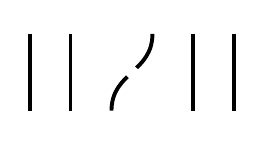
\begin{tikzpicture}[
    x=0.65cm,
    y=0.65cm,
    baseline={(current bounding box.center)}
]
  \draw[line width=1.4] (-2.00, 0.00) to (-2.00, -1.50);
  \draw[line width=1.4] (-1.20, 0.00) to (-1.20, -1.50);
  \draw[line width=1.4] (1.20, 0.00) to (1.20, -1.50);
  \draw[line width=1.4] (2.00, 0.00) to (2.00, -1.50);
  \draw[line width=1.4] (0.40, 0.00) .. controls (0.40, -0.75) and (-0.40, -0.75) .. (-0.40, -1.50);
  \draw[line width=4.5, white] (-0.40, 0.00) .. controls (-0.40, -0.75) and (0.40, -0.75) .. (0.40, -1.50);
\end{tikzpicture}%
}



\newcommand{\FusionTreeThreeLabelRight}[5]{%
\begin{tikzpicture}[
    x=0.65cm,
    y=0.65cm,
    baseline={(current bounding box.center)}
]
    % Incoming leaves
    \coordinate (A) at (1.6,2);
    \coordinate (B) at (0.8,2);
    \coordinate (C) at (0,2);
    \coordinate (D) at (0.4,0.5);

    \coordinate (Vone) at (1.2,1.5);
    \coordinate (Vtwo) at (0.8,1);

    \draw[fusionarrow] (A) -- (Vone);
    \draw[fusionarrow] (B) -- (Vone);
    \draw[fusionarrow] (Vone) -- (Vtwo);
    \draw[fusionarrow] (C) -- (Vtwo);
    \draw[fusionarrow] (Vtwo) -- (D);

    \node[right=1.5pt, font=\scriptsize] at (Vone) {$#5$};

    \node[above, font=\scriptsize] at (A) {$#3$};
    \node[above, font=\scriptsize] at (B) {$#2$};
    \node[above, font=\scriptsize] at (C) {$#1$};
    \node[right, font=\scriptsize] at (D) {$#4$};
\end{tikzpicture}%
}

\begin{document}


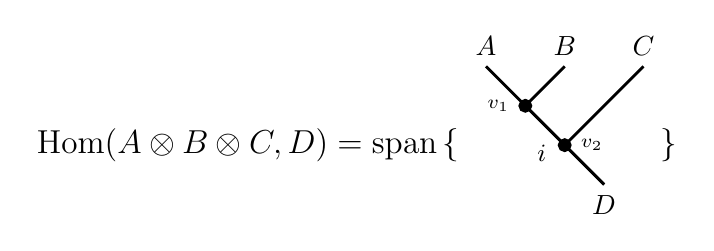
\begin{tikzpicture}[line width=1pt, node distance=1cm]

    \node at (-1.5, 1) {\large $\mathrm{Hom}(A \otimes B \otimes C, D) = \mathrm{span} \left\{ \vphantom{\sum} \right.$};

    \begin{scope}[shift={(1.5,0)}]
        % Incoming leaves
        \coordinate (A) at (0,2);
        \coordinate (B) at (1,2);
        \coordinate (C) at (2,2);
        \coordinate (D) at (1.5,0.5);
        
        \coordinate (V1) at (0.5, 1.5); 
        \coordinate (V2) at (1.0, 1); % 
        
        \draw (A) -- (D);
        \draw (B) -- (V1);
        \draw (V1) -- (V2);
        \draw (C) -- (V2);
        \draw (V2) -- (D);

        \filldraw (V1) circle (2pt) node[left=2pt, font=\scriptsize] {$v_1$};
        \filldraw (V2) circle (2pt) node[right=2pt, font=\scriptsize] {$v_2$};

        \node[above] at (A) {$A$};
        \node[above] at (B) {$B$};
        \node[above] at (C) {$C$};
        \node[below] at (D) {$D$};
        
        \node[left, font=\small] at (0.9,0.9) {$i$};
    \end{scope}


    \node at (3.8, 1) {\large $\left. \vphantom{\sum} \right\}$};

\end{tikzpicture}


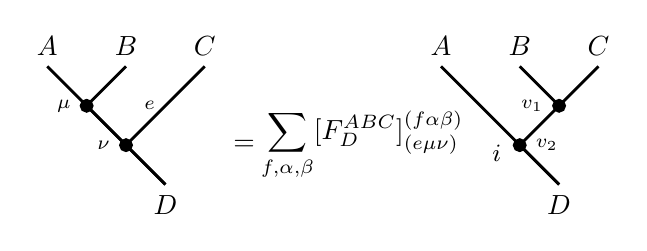
\begin{tikzpicture}[line width=1pt, node distance=1cm]

        % Incoming leaves
        \coordinate (A) at (0,2);
        \coordinate (B) at (1,2);
        \coordinate (C) at (2,2);
        \coordinate (D) at (1.5,0.5);
        
        \coordinate (V1) at (0.5, 1.5); 
        \coordinate (V2) at (1.0, 1); % 
        
        \draw (A) -- (D);
        \draw (B) -- (V1);
        \draw (V1) -- (V2);
        \draw (C) -- (V2);
        \draw (V2) -- (D);

        \filldraw (V1) circle (2pt) node[left=2pt, font=\scriptsize] {$\mu$};
        \filldraw (V2) circle (2pt) node[left=2pt, font=\scriptsize] {$\nu$};

        \node[above] at (A) {$A$};
        \node[above] at (B) {$B$};
        \node[above] at (C) {$C$};
        \node[below] at (D) {$D$};
        
        \node[left, font=\scriptsize] at (1.5,1.5) {$e$};
        \node at (2.5,1) {$=$};
        \node at (4,1) {$\displaystyle\sum_{f,\alpha,\beta} [F^{ABC}_{D}]_{(e \mu \nu)}^{(f \alpha \beta)} $};

        \begin{scope}[shift={(5,0)}]
        % Incoming leaves
        \coordinate (A) at (0,2);
        \coordinate (B) at (1,2);
        \coordinate (C) at (2,2);
        \coordinate (D) at (1.5,0.5);
        
        \coordinate (V2) at (1.0, 1); 
        \coordinate (V1) at (1.5, 1.5); % 
        
        \draw (A) -- (D);
        \draw (B) -- (V1);
        \draw (V1) -- (V2);
        \draw (C) -- (V1);
        \draw (V2) -- (D);

        \filldraw (V1) circle (2pt) node[left=2pt, font=\scriptsize] {$v_1$};
        \filldraw (V2) circle (2pt) node[right=2pt, font=\scriptsize] {$v_2$};

        \node[above] at (A) {$A$};
        \node[above] at (B) {$B$};
        \node[above] at (C) {$C$};
        \node[below] at (D) {$D$};
        
        \node[left, font=\small] at (0.9,0.9) {$i$};
    \end{scope}

\end{tikzpicture}

\begin{equation*}
  \vert 0 \rangle =
\raisebox{-20pt}{
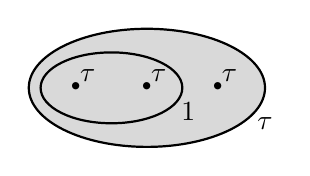
\begin{tikzpicture}[scale=1.5]
    \fill[gray!30] (3,0) ellipse (1 and 0.5);
    \draw[thick] (3,0) ellipse (1 and 0.5);
    
    \draw[thick] (2.7,0) ellipse (0.6 and 0.3);
    \node at (3.35,-0.2) {$1$};
    \node[scale=2.5] at (2.4, 0) {$\cdot$};
    \node at (2.5,0.1) {$\tau$};
    \node[scale=2.5] at (3.0, 0) {$\cdot$};
    \node at (3.1,0.1) {$\tau$};
    \node[scale=2.5] at (3.6, 0) {$\cdot$};
    \node at (3.7,0.1) {$\tau$};
    \node at (4.0,-0.3) {$\tau$};
\end{tikzpicture}
} 
\quad
\vert 1 \rangle = 
\raisebox{-20pt}{
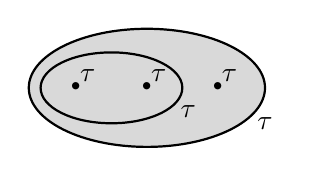
\begin{tikzpicture}[scale=1.5]    
    \fill[gray!30] (3,0) ellipse (1 and 0.5);
    \draw[thick] (3,0) ellipse (1 and 0.5);
    
    \draw[thick] (2.7,0) ellipse (0.6 and 0.3);
    \node at (3.35,-0.2) {$\tau$};

    \node[scale=2.5] at (2.4, 0) {$\cdot$};
    \node at (2.5,0.1) {$\tau$};
    \node[scale=2.5] at (3.0, 0) {$\cdot$};
    \node at (3.1,0.1) {$\tau$};
    \node[scale=2.5] at (3.6, 0) {$\cdot$};
    \node at (3.7,0.1) {$\tau$};
    \node at (4.0,-0.3) {$\tau$};
\end{tikzpicture}
}
\quad 
\vert NC \rangle =
\raisebox{-20pt}{
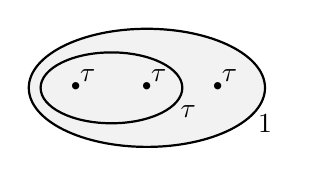
\begin{tikzpicture}[scale=1.5]

    \fill[gray!10] (3,0) ellipse (1 and 0.5);
    \draw[thick] (3,0) ellipse (1 and 0.5);
    
    \draw[thick] (2.7,0) ellipse (0.6 and 0.3);
    \node at (3.35,-0.2) {$\tau$};
    \node[scale=2.5] at (2.4, 0) {$\cdot$};
    \node at (2.5, 0.1) {$\tau$};
    \node[scale=2.5] at (3.0, 0) {$\cdot$};
    \node at (3.1,0.1) {$\tau$};
    \node[scale=2.5] at (3.6, 0) {$\cdot$};
    \node at (3.7,0.1) {$\tau$};
    \node at (4.0,-0.3) {$1$};

\end{tikzpicture}
}
\end{equation*}

\begin{tikzpicture}
    
\end{tikzpicture}
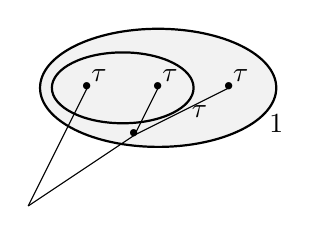
\begin{tikzpicture}[scale=1.5]

    \fill[gray!10] (3,0) ellipse (1 and 0.5);
    \draw[thick] (3,0) ellipse (1 and 0.5);
    
    \draw[thick] (2.7,0) ellipse (0.6 and 0.3);
    \node at (3.35,-0.2) {$\tau$};
    \node[scale=2.5] at (2.4, 0) {$\cdot$};
    \node at (2.5, 0.1) {$\tau$};
    \node[scale=2.5] at (3.0, 0) {$\cdot$};
    \node at (3.1,0.1) {$\tau$};
    \node[scale=2.5] at (3.6, 0) {$\cdot$};
    \node at (3.7,0.1) {$\tau$};
    \node at (4.0,-0.3) {$1$};
    \node[scale=2.5] at (2.8, -0.4) {$\cdot$};
    \draw (3.0, 0.0) -- (2.8, -0.4);
    \draw (3.6, 0.0) -- (2.8, -0.4); 
    \draw (2.8, -0.4) -- (1.9, -1.0);
    \draw (2.4, 0.0) -- (1.9, -1.0);
\end{tikzpicture}

% https://q.uiver.app/#q=WzAsMTQsWzAsMCwiKEFcXG90aW1lcyBCKVxcb3RpbWVzIEMiXSxbMiwwLCJBIFxcb3RpbWVzIChCIFxcb3RpbWVzIEMpIl0sWzAsMiwiSG9tKChBXFxvdGltZXMgQikgXFxvdGltZXMgQywgRCkiXSxbMiwyLCJIb20oQVxcb3RpbWVzIChCIFxcb3RpbWVzIEMpLCBEKSJdLFswLDUsIlxcZGlzcGxheXN0eWxlXFxiaWdvcGx1c19jIFZee0FCfV9jIFxcb3RpbWVzIFZee2NDfV9EIl0sWzIsNSwiXFxkaXNwbGF5c3R5bGVcXGJpZ29wbHVzX2MgVl57QWN9X0QgXFxvdGltZXMgVl57QkN9X2MiXSxbMSwyLCJcXGNvbmciXSxbMSw0LCJcXGNvbmciXSxbMCw2LCJcXHZlcnQgKEEsQik7YztcXG11XFxyYW5nbGUgXFxvdGltZXMgXFx2ZXJ0IGMsQzsgRDsgXFxudSBcXHJhbmdsZSJdLFsyLDYsIlxcc3VtX3tmLFxcYWxwaGEsXFxiZXRhfSBbRl9EXntBQkN9XV97KGNcXG11XFxudSl9XnsoZlxcYWxwaGFcXGJldGEpfSBcXHZlcnQgQSxmO0Q7XFxiZXRhXFxyYW5nbGUgXFxvdGltZXMgXFx2ZXJ0IEIsQzsgZjsgXFxhbHBoYSBcXHJhbmdsZSJdLFsxLDUsIlxcdGV4dHtjaG9pY2Ugb2YgYmFzaXN9Il0sWzAsNCwiXFxkaXNwbGF5c3R5bGVcXGJpZ29wbHVzX2MgSG9tKEEgXFxvdGltZXMgQiwgYykgXFxvdGltZXMgSG9tKGMgXFxvdGltZXMgQywgRCkiXSxbMiw0LCJcXGRpc3BsYXlzdHlsZVxcYmlnb3BsdXNfe2QgXFxpbiBJcnIoXFxtYXRoc2Z7Q2F0fSl9IEhvbShBIFxcb3RpbWVzIGQsIEQpIFxcb3RpbWVzIEhvbShCIFxcb3RpbWVzIEMsIGQpIl0sWzEsMywiXFx0ZXh0e3NlbWlzaW1wbGljaXR5fSJdLFswLDIsIkhvbSgtLEQpIiwxXSxbMSwzLCJIb20oLSxEKSIsMV0sWzAsMSwiXFxhbHBoYV97QUJDfSJdLFs0LDgsIlxcaW4iLDMseyJzdHlsZSI6eyJib2R5Ijp7Im5hbWUiOiJub25lIn0sImhlYWQiOnsibmFtZSI6Im5vbmUifX19XSxbOCw5LCIiLDEseyJsZXZlbCI6Miwic3R5bGUiOnsiaGVhZCI6eyJuYW1lIjoibm9uZSJ9fX1dLFsyLDExLCJcXHVuZGVyc2V0e1xcdGV4dHtzZW1pc2ltcGxpY2l0eX19e1xcY29uZ30iLDMseyJzdHlsZSI6eyJib2R5Ijp7Im5hbWUiOiJub25lIn0sImhlYWQiOnsibmFtZSI6Im5vbmUifX19XSxbMywxMiwiXFx1bmRlcnNldHtcXHRleHR7c2VtaXNpbXBsaWNpdHl9fXtcXGNvbmd9IiwzLHsic3R5bGUiOnsiYm9keSI6eyJuYW1lIjoibm9uZSJ9LCJoZWFkIjp7Im5hbWUiOiJub25lIn19fV0sWzExLDQsIlxcY29uZyIsMyx7InN0eWxlIjp7ImJvZHkiOnsibmFtZSI6Im5vbmUifSwiaGVhZCI6eyJuYW1lIjoibm9uZSJ9fX1dLFsxMiw1LCJcXGNvbmciLDMseyJzdHlsZSI6eyJib2R5Ijp7Im5hbWUiOiJub25lIn0sImhlYWQiOnsibmFtZSI6Im5vbmUifX19XSxbNSw5LCJcXGluIiwzLHsic3R5bGUiOnsiYm9keSI6eyJuYW1lIjoibm9uZSJ9LCJoZWFkIjp7Im5hbWUiOiJub25lIn19fV0sWzE2LDYsIlxcdGV4dHtZb25lZGEtbGlmdGluZ30iLDEseyJzaG9ydGVuIjp7InNvdXJjZSI6MjB9LCJzdHlsZSI6eyJib2R5Ijp7Im5hbWUiOiJub25lIn0sImhlYWQiOnsibmFtZSI6Im5vbmUifX19XV0=
\[\begin{tikzcd}
	{(A\otimes B)\otimes C} && {A \otimes (B \otimes C)} \\
	\\
	{Hom((A\otimes B) \otimes C, D)} & \cong & {Hom(A\otimes (B \otimes C), D)} \\
	& {\text{semisimplicity}} \\
	{\displaystyle\bigoplus_c Hom(A \otimes B, c) \otimes Hom(c \otimes C, D)} & \cong & {\displaystyle\bigoplus_{d \in Irr(\mathsf{Cat})} Hom(A \otimes d, D) \otimes Hom(B \otimes C, d)} \\
	{\displaystyle\bigoplus_c V^{AB}_c \otimes V^{cC}_D} & {\text{choice of basis}} & {\displaystyle\bigoplus_c V^{Ac}_D \otimes V^{BC}_c} \\
	{\vert (A,B);c;\mu\rangle \otimes \vert c,C; D; \nu \rangle} && {\sum_{f,\alpha,\beta} [F_D^{ABC}]_{(c\mu\nu)}^{(f\alpha\beta)} \vert A,f;D;\beta\rangle \otimes \vert B,C; f; \alpha \rangle}
	\arrow[""{name=0, anchor=center, inner sep=0}, "{\alpha_{ABC}}", from=1-1, to=1-3]
	\arrow["{Hom(-,D)}"{description}, from=1-1, to=3-1]
	\arrow["{Hom(-,D)}"{description}, from=1-3, to=3-3]
	\arrow["{\underset{\text{semisimplicity}}{\cong}}"{marking, allow upside down}, draw=none, from=3-1, to=5-1]
	\arrow["{\underset{\text{semisimplicity}}{\cong}}"{marking, allow upside down}, draw=none, from=3-3, to=5-3]
	\arrow["\cong"{marking, allow upside down}, draw=none, from=5-1, to=6-1]
	\arrow["\cong"{marking, allow upside down}, draw=none, from=5-3, to=6-3]
	\arrow["\in"{marking, allow upside down}, draw=none, from=6-1, to=7-1]
	\arrow["\in"{marking, allow upside down}, draw=none, from=6-3, to=7-3]
	\arrow[equals, from=7-1, to=7-3]
	\arrow["{\text{Yoneda-lifting}}"{description}, draw=none, from=0, to=3-2]
\end{tikzcd}\]


Let $f : E \to A \otimes B$ and $g : D \to E \otimes C$.

%\newcommand{\blue}[1]{\textcolor{blue}{#1}}
%\newcommand{\green}[1]{\textcolor{green}{#1}}

% https://q.uiver.app/#q=WzAsMTIsWzAsMCwiKEFcXG90aW1lcyBCKVxcb3RpbWVzIEMiXSxbMiwwLCJBIFxcb3RpbWVzIChCIFxcb3RpbWVzIEMpIl0sWzAsMiwiSG9tKChBXFxvdGltZXMgQikgXFxvdGltZXMgQywgRCkiXSxbMiwyLCJIb20oQVxcb3RpbWVzIChCIFxcb3RpbWVzIEMpLCBEKSJdLFswLDUsIlxcZGlzcGxheXN0eWxlXFxiaWdvcGx1c19jIFZee0FCfV9jIFxcb3RpbWVzIFZee2NDfV9EIl0sWzIsNSwiXFxkaXNwbGF5c3R5bGVcXGJpZ29wbHVzX2MgVl57QWN9X0QgXFxvdGltZXMgVl57QkN9X2MiXSxbMSw0LCJcXGNvbmciXSxbMCw2LCJcXHVuZGVyc2V0e1xcYmx1ZXtcXG11IFxcaW4gMSxcXGxkb3RzLCBOXntBQn1fY30gXFxxdWFkIFxcYmx1ZXtcXG51IFxcaW4gMSxcXGxkb3RzLE5ee2NDLER9fX17XFx2ZXJ0IChBLEIpO2M7XFxtdVxccmFuZ2xlIFxcb3RpbWVzIFxcdmVydCBjLEM7IEQ7IFxcbnUgXFxyYW5nbGV9Il0sWzIsNiwiXFxkaXNwbGF5c3R5bGVcXHN1bV97ZixcXGFscGhhLFxcYmV0YX0gW0ZfRF57QUJDfV1feyhjXFxtdVxcbnUpfV57KGZcXGFscGhhXFxiZXRhKX0gXFx2ZXJ0IEEsZjtEO1xcYmV0YVxccmFuZ2xlIFxcb3RpbWVzIFxcdmVydCBCLEM7IGY7IFxcYWxwaGEgXFxyYW5nbGUiXSxbMCw0LCJcXGRpc3BsYXlzdHlsZVxcYmlnb3BsdXNfe2NcXGluIElycihDQVQpfSBIb20oQSBcXG90aW1lcyBCLCBjKSBcXG90aW1lcyBIb20oYyBcXG90aW1lcyBDLCBEKSJdLFsyLDQsIlxcZGlzcGxheXN0eWxlXFxiaWdvcGx1c197ZCBcXGluIElycihcXG1hdGhzZntDYXR9KX0gSG9tKEEgXFxvdGltZXMgZCwgRCkgXFxvdGltZXMgSG9tKEIgXFxvdGltZXMgQywgZCkiXSxbMSw1LCJcXGNvbmciXSxbMCwyLCJIb20oLSxEKSIsMV0sWzEsMywiSG9tKC0sRCkiLDFdLFswLDEsIlxcdW5kZXJzZXR7XFxzaW19e1xcYWxwaGFfe0FCQ319Il0sWzQsNywiXFxpbiIsMyx7InN0eWxlIjp7ImJvZHkiOnsibmFtZSI6Im5vbmUifSwiaGVhZCI6eyJuYW1lIjoibm9uZSJ9fX1dLFs3LDgsIlxcdW5kZXJzZXR7XFxncmVlbntcXHRleHR7Nmotc3ltYm9sc319fXtGXntBQkN9X0R9IiwxLHsic2hvcnRlbiI6eyJzb3VyY2UiOjEwLCJ0YXJnZXQiOjEwfX1dLFsyLDksIlxcdW5kZXJzZXR7XFx0ZXh0e1xcZ3JlZW57c2VtaXNpbXBsaWNpdHl9fX17XFxjb25nfSIsMyx7InN0eWxlIjp7ImJvZHkiOnsibmFtZSI6Im5vbmUifSwiaGVhZCI6eyJuYW1lIjoibm9uZSJ9fX1dLFszLDEwLCJcXHVuZGVyc2V0e1xcdGV4dHtcXGdyZWVue3NlbWlzaW1wbGljaXR5fX19e1xcY29uZ30iLDMseyJvZmZzZXQiOi0yLCJzdHlsZSI6eyJib2R5Ijp7Im5hbWUiOiJub25lIn0sImhlYWQiOnsibmFtZSI6Im5vbmUifX19XSxbOSw0LCI9IiwzLHsic3R5bGUiOnsiYm9keSI6eyJuYW1lIjoibm9uZSJ9LCJoZWFkIjp7Im5hbWUiOiJub25lIn19fV0sWzEwLDUsIj0iLDMseyJzdHlsZSI6eyJib2R5Ijp7Im5hbWUiOiJub25lIn0sImhlYWQiOnsibmFtZSI6Im5vbmUifX19XSxbNSw4LCJcXGluIiwzLHsic3R5bGUiOnsiYm9keSI6eyJuYW1lIjoibm9uZSJ9LCJoZWFkIjp7Im5hbWUiOiJub25lIn19fV0sWzIsMywiXFx1bmRlcnNldHtcXHNpbX17XFxhbHBoYV97QSxCLEN9fSJdLFsyLDMsIlxcc21hbGxcXGdyZWVue1xcdGV4dHthc3NvY2lhdG9yIGluZHVjZXMgaXNvbW9ycGhpbXMgdW5kZXIgeW9uZWRhfX0iLDAseyJvZmZzZXQiOjUsInN0eWxlIjp7ImJvZHkiOnsibmFtZSI6Im5vbmUifSwiaGVhZCI6eyJuYW1lIjoibm9uZSJ9fX1dXQ==
\[\begin{tikzcd}
	{(A\otimes B)\otimes C} && {A \otimes (B \otimes C)} \\
	\\
	{Hom((A\otimes B) \otimes C, D)} && {Hom(A\otimes (B \otimes C), D)} \\
	\\
	{\displaystyle\bigoplus_{c\in Irr(CAT)} Hom(A \otimes B, c) \otimes Hom(c \otimes C, D)} & \cong & {\displaystyle\bigoplus_{d \in Irr(\mathsf{Cat})} Hom(A \otimes d, D) \otimes Hom(B \otimes C, d)} \\
	{\displaystyle\bigoplus_c V^{AB}_c \otimes V^{cC}_D} & \cong & {\displaystyle\bigoplus_c V^{Ac}_D \otimes V^{BC}_c} \\
	{\underset{\blue{\mu \in 1,\ldots, N^{AB}_c} \quad \blue{\nu \in 1,\ldots,N^{cC,D}}}{\vert (A,B);c;\mu\rangle \otimes \vert c,C; D; \nu \rangle}} && {\displaystyle\sum_{f,\alpha,\beta} [F_D^{ABC}]_{(c\mu\nu)}^{(f\alpha\beta)} \vert A,f;D;\beta\rangle \otimes \vert B,C; f; \alpha \rangle} \\
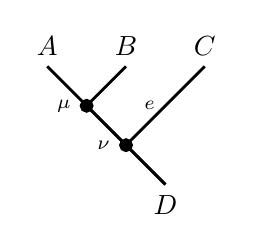
\begin{tikzpicture}[line width=1pt, node distance=1cm]
    % First diagram
    \coordinate (A) at (0,2);
    \coordinate (B) at (1,2);
    \coordinate (C) at (2,2);
    \coordinate (D) at (1.5,0.5);

    \coordinate (V1) at (0.5,1.5);
    \coordinate (V2) at (1.0,1);

    \draw (A) -- (D);
    \draw (B) -- (V1);
    \draw (V1) -- (V2);
    \draw (C) -- (V2);
    \draw (V2) -- (D);

    \filldraw (V1) circle (2pt) node[left=2pt,font=\scriptsize] {$\mu$};
    \filldraw (V2) circle (2pt) node[left=2pt,font=\scriptsize] {$\nu$};

    \node[above] at (A) {$A$};
    \node[above] at (B) {$B$};
    \node[above] at (C) {$C$};
    \node[below] at (D) {$D$};

    \node[left,font=\scriptsize] at (1.5,1.5) {$e$};
\end{tikzpicture}
& =  &
\hspace{-1.8cm}%
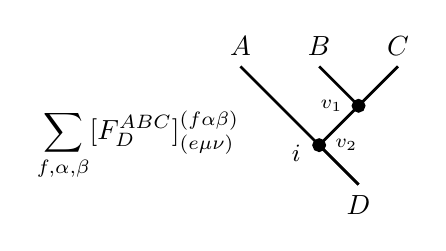
\begin{tikzpicture}[line width=1pt, node distance=1cm, xshift=-2cm]
    \begin{scope}[xshift=-2]
        
    \node at (-1.3,1) 
    {$\displaystyle\sum_{f,\alpha,\beta}
    [F^{ABC}_{D}]_{(e\mu\nu)}^{(f\alpha\beta)}$};

    \coordinate (A) at (0,2);
    \coordinate (B) at (1,2);
    \coordinate (C) at (2,2);
    \coordinate (D) at (1.5,0.5);

    \coordinate (V2) at (1.0,1);
    \coordinate (V1) at (1.5,1.5);

    \draw (A) -- (D);
    \draw (B) -- (V1);
    \draw (V1) -- (V2);
    \draw (C) -- (V1);
    \draw (V2) -- (D);

    \filldraw (V1) circle (2pt) node[left=2pt,font=\scriptsize] {$v_1$};
    \filldraw (V2) circle (2pt) node[right=2pt,font=\scriptsize] {$v_2$};

    \node[above] at (A) {$A$};
    \node[above] at (B) {$B$};
    \node[above] at (C) {$C$};
    \node[below] at (D) {$D$};

    \node[left,font=\small] at (0.9,0.9) {$i$};
    \end{scope}
\end{tikzpicture}
	\arrow["{\underset{\sim}{\alpha_{ABC}}}", from=1-1, to=1-3]
	\arrow["{Hom(-,D)}"{description}, from=1-1, to=3-1]
	\arrow["{Hom(-,D)}"{description}, from=1-3, to=3-3]
	\arrow["{\underset{\sim}{\alpha_{A,B,C}}}", from=3-1, to=3-3]
	\arrow["{\green{\text{associator induces isomorphims under yoneda}}}", shift right=5, draw=none, from=3-1, to=3-3]
	\arrow["{\underset{\text{\green{semisimplicity}}}{\cong}}"{marking, allow upside down}, draw=none, from=3-1, to=5-1]
	\arrow["{\underset{\text{\green{semisimplicity}}}{\cong}}"{marking, allow upside down}, shift left=2, draw=none, from=3-3, to=5-3]
	\arrow["{=}"{marking, allow upside down}, draw=none, from=5-1, to=6-1]
	\arrow["{=}"{marking, allow upside down}, draw=none, from=5-3, to=6-3]
	\arrow["\in"{marking, allow upside down}, draw=none, from=6-1, to=7-1]
	\arrow["\in"{marking, allow upside down}, draw=none, from=6-3, to=7-3]
	\arrow["{\underset{\green{\text{6j-symbols}}}{F^{ABC}_D}}"{description},  from=7-1, to=7-3]
\end{tikzcd}\]
\end{document}